%! Author = florian
%! Date = 25.05.23


\section{Eco-Friendly Consensus Mechanisms}\label{sec:eco-friendly-consensus-mechanisms}
This section will describe and compare alternative consensus mechanisms.
Currently, around 60\% of the consensus mechanisms used in blockchains is the proof-of-work (PoW) consensus mechanism.
As described in Section~\ref{sec:introduction}, the PoW consensus mechanism requires miners to solve complex mathematical puzzles to create blocks on the blockchain, resulting in high energy consumption and negative environmental impact~\cite{overview-of-sustainablity-blockchains, moralis-pow-enery-consumption}.

By transitioning to alternative consensus mechanisms, blockchains can significantly reduce their energy consumption.
This section will describe these alternative consensus mechanisms~\cite{4-ways-to-counter-blockchains-energy-consumption}.

\subsection{Proof of Stake}\label{subsec:proof-of-stake}
Proof of stake (PoS) is the second most widely used consensus algorithm, following proof of work.
Unlike PoW, the PoS consensus algorithm does not require miners to create blocks for the blockchain.
Instead, participants who wish to create blocks must stake a certain amount of the network's tokens.
These participants, known as validators, lock their coins in the stake, rendering them unavailable for transactions.
If a validator wants to access the tokens in their stake, they must stop being a validator and the tokens cannot be use immediately after removing them from the stake.
In other words, they have a cool-down time.
The number of blocks validators can create is limited by the size of their stake.
Validators receive transaction fees associated with the transactions in the block, but they do not receive mining rewards~\cite{bitpanda-pos}.

Another aspect of PoS is the penalty mechanism.
If a participant acts maliciously or remains offline, their stake can be slashed, resulting in the removal of the staked tokens from their account~\cite{bitpanda-pos}.

The deterministic nature of PoS means that the creator of a block is selected based on the size of their stake.
However, this can lead to unwanted centralization, as participants with more tokens have an advantage over those with fewer tokens.
To mitigate centralization, other selection methods are employed, such as:

\begin{itemize}
    \item \textbf{Stationary Time}: Validators are selected based on the duration of time their cryptocurrency has been locked up in the network~\cite{bitpanda-pos}.
    \item \textbf{Coin Age}: Validators are selected based on the product of their stake and the duration of time the tokens have been held in the network~\cite{bitflyer-glossary}.
    \item \textbf{Randomized Block Selection}: Validators are selected based on a pseudorandom function that combines their stake with other factors, such as the hash of the previous block~\cite{cryptonews-pos}.
\end{itemize}

\subsubsection{Pros and Cons of Proof of Stake}
As mentioned earlier, proof-of-stake is more energy-efficient since no actual calculations are required.
It also offers higher throughput compared to proof-of-work and has a lower entry barrier, as specialized hardware is not necessary for mining blocks.
An interesting aspect of proof of stake is that it reduces centralization risks posed by mining farms, as more nodes can participate, thereby decreasing centralization~\cite{bitpanda-pos}.

However, proof-of-stake enables centralization in that sense, that validators with higher stakes hold an advantage over participants with lesser stakes.
Additionally, proof of stake is not as mature as proof of work, and further research is needed to determine its viability as an alternative solution~\cite{insider-pos-vs-pow}.

One challenge of proof-of-stake is the ``nothing at stake'' problem.
Since block creation does not require any actual work, participants could create multiple parallel chains to gain transaction fees.
The solution to this problem is to penalize participants who create multiple parallel blocks.

\subsection{Proof of Capacity}\label{subsec:proof-of-capacity}
Proof-of-capacity is a consensus mechanism that utilizes empty storage space instead of CPUs or GPUs to create blocks.
Miners, also known as farmers in this case, employ HDDs and SSDs to farm blocks.
The empty storage space is divided into plots, where each plot represents a file on the storage device.
Plots are filled with precalculated proof-of-work functions.
When a new block needs to be farmed, farmers simply scan their plots for the correct one and proceed with farming that plot.

The more storage space allocated by a node operator on their hard drive, the higher the likelihood of finding a matching hash value from a predetermined list, thereby increasing their chances of winning the mining reward.
While this mechanism requires a large amount of free space on a hard drive, it does not consume significant amounts of energy to create new blocks~\cite{chia-whitepaper,geeksforgeeks-poc}.

There are a few other consensus mechanisms that are similar to proof of capacity, such as:

\begin{itemize}
    \item \textbf{Proof of Space}: In this consensus mechanism, the prover (farmer) sends a piece of data to a verifier to demonstrate that the farmer has reserved a certain amount of space on their storage device.
    It shares similarities with proof of stake, as described in Subsection~\ref{subsec:proof-of-stake}, but instead of using tokens, it utilizes storage space.
    \item \textbf{Conditional Proof of Capacity}: This consensus mechanism combines proof-of-work, proof of stake (described in Subsection~\ref{subsec:proof-of-stake}), and proof-of-capacity.
    Miners can earn a higher income by pledging additional tokens, similar to proof of stake.
\end{itemize}

\subsubsection{Pros and Cons of Proof of Capacity}
Like the other consensus mechanisms mentioned in this section, proof of capacity is more eco-friendly than proof of work.
Additionally, it offers the advantage of being accessible to anyone with free storage space.
This is particularly useful when a farmer has unused storage capacity for future purposes.
Moreover, there is no need for equipment upgrades, as even old storage devices can effectively store data.
After farming, the farmer can wipe the storage device and repurpose it for other storage needs.

However, there are some limitations.
Storage devices have finite capacities, so farmers may need to purchase additional storage devices to farm more efficiently.
Moreover, there is a risk of centralization if a limited number of miners control the majority of storage space.
Lastly, in the event of storage device failure, there is a possibility of losing stored data and mining rewards~\cite{geeksforgeeks-poc}.

\subsection{Proof of Space and Time}\label{subsec:proof-of-space-and-time}
Another alternative consensus mechanism is proof of space and time (PoST).
It requires participants to utilize storage space to validate transactions and is intended to be more energy-efficient than proof-of-work and proof-of-stake.

In more detail, proof-of-space-and-time consists of two different consensus mechanisms that are combined.
First, proof-of-space reserves hard-drive space for mining blocks, which is also described in Subsection~\ref{subsec:proof-of-capacity}.
Since proof-of-space requires little to no time for lookup, a second consensus mechanism called proof-of-time is introduced.
Proof of time introduces a small delay between blocks using a verifiable delay function (VDF).
The VDF takes a certain time to compute but is fast to verify, similar to proof-of-work.
Unlike proof-of-work, it requires sequential computation, eliminating the advantage of using parallel GPUs, CPUs or ASICs.
The workload is adjusted over time to ensure the creation of the same number of blocks within a given timespan.
This delay prevents miners from receiving additional rewards when mining with large amounts of storage space.
However, participants can still run multiple nodes~\cite{supraoracles-post,chia-whitepaper}.

\subsubsection{Pros and Cons of Proof of Space and Time}
As previously mentioned, PoST is more energy-efficient as it utilizes unused storage space rather than computational power.
The hardware requirements for running a validator node are also lower, as it only requires free storage space.

One major disadvantage of PoST is the increased wear on HDDs and SSDs.
It can significantly reduce the lifespan of a hard drive to as little as 40 days, compared to the usual lifespan of a decade.
This implies that while PoST itself requires less energy, it may not be an eco-friendly solution, as validators will need to purchase new hard drives more frequently, leading to increased waste generation.
In comparison, the lifespan of a GPU used for mining cryptocurrencies is typically around three to five years, significantly longer than the lifespan of a hard drive used for farming.
Therefore, while PoST is more energy-efficient, it is not necessarily better for the environment~\cite{euronews-chia, devicetest-gpu-lifespan, supraoracles-post}.

\subsection{Proof of Authority}\label{subsec:proof-of-authority}
The proof-of-authority consensus mechanism differs significantly from the other consensus algorithms already described in this section.
It is primarily suitable for private blockchains.
In proof-of-authority, not everyone can become a validator.
Instead, validators are preselected based on their reputation, rather than using stake or time and space.
To become a validator, candidates need to undergo identity verification and be willing to stake money and/or their reputation.
Usually, a rigorous selection process is implemented to filter out questionable candidates~\cite{coindesk-poa}.

\subsubsection{Pros and Cons of Proof of Authority}
There are several pros and cons associated with proof-of-authority.
One advantage of a blockchain based on proof of authority is its ability to process a higher number of transactions per second, as there is no need to perform proof-of-work calculations for every block created by a validator.
Blockchains utilizing proof-of-authority are also more resistant to 51\% attacks, as all validators have undergone rigorous vetting.
Validators do not require special hardware to build blocks, unlike in proof-of-work or proof-of-space-and-time, as mentioned in Subsection~\ref{subsec:proof-of-space-and-time}.

A significant disadvantage is the centralization of the blockchain.
Due to the need to check and identify each potential validator, not every participant in the blockchain can become one.
Consequently, the decentralized nature of the blockchain, as illustrated in Figure~\ref{fig:centralization-of-proof-of-authority}, is compromised.
Immutability is a key aspect of blockchains, which makes them resilient to censorship, ensuring availability for everyone.
By centralizing the validators, these essential characteristics of blockchains are diminished.
It becomes easier to block specific participants or manipulate the blockchain if the validators wish to do so.

Since the validator nodes are publicly known, they are vulnerable to manipulation themselves.
External actors could attempt to influence validators to act dishonestly or destructively~\cite{insidecrypto-poa,coindesk-poa}.


\begin{figure}[h]
    \centering
    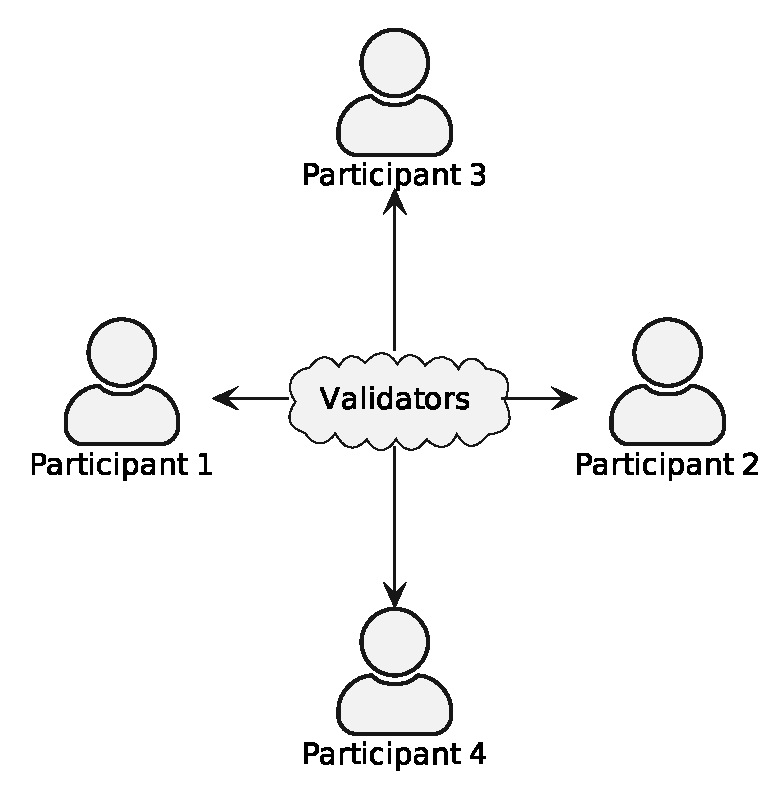
\includegraphics[scale=0.5]{img/proof-of-authority-0}
    \caption{Centralization of Proof of Authority}
    \label{fig:centralization-of-proof-of-authority}
\end{figure}

